\documentclass[a4paper]{article}
%\include{amsfonts}
\usepackage{amssymb,amsmath,amsthm,latexsym,epsfig,euscript,multicol}
\usepackage{enumitem}
\usepackage{graphicx}
\usepackage{float}
\usepackage[margin=2cm]{geometry}
\usepackage{hyperref}

%\usepackage[utf8x]{inputenc}
\usepackage[spanish]{babel}% idioma castellano
\graphicspath{{fig/}}

% Caracteres especiales
\def\A{\mathbb{A}}
\def\C{\mathbb{C}}
\def \N{\mathbb{N}}
\def \P{\mathbb{P}}
\def \Q{\mathbb{Q}}
\def \R{\mathbb{R}}
\def \Z{\mathbb{Z}}

\def\zC{\mathbb{C}}
\def \zN{\mathbb{N}}

\def \zQ{\mathbb{Q}}
\def \zR{\mathbb{R}}
\def \zZ{\mathbb{Z}}

%  Ejercicio:
\newtheorem{ejer}{Unidad}
\newcommand{\bej}{\begin{ejer} \rm}
\newcommand{\fej}{\end{ejer}}


%
\def\d{\displaystyle}

%Encabezado y pie de página
\usepackage{fancyhdr} % Headers and footers
\setlength{\headwidth}{16.5cm}
\pagestyle{fancy} % All pages have headers and footers


\renewcommand{\headrulewidth}{1.5pt}


\renewcommand{\footrulewidth}{1.5pt}

\fancyhead{} % Blank out the default header
\fancyfoot{} % Blank out the default footer
\fancyhead[L]{Taller de Programación para ciencias exactas} % Custom header text
\fancyhead[R]{{\small Departamento de Física, FCEN, UBA}}% Custom header text
\fancyfoot[RO,LE]{\thepage} % Custom footer text
\fancyfoot[LO,RE]{FIFA}


%\topmargin-2cm \vsize 29.5cm \hsize 21cm
%\setlength{\textwidth}{16.5cm} \setlength{\textheight}{23.5cm}
%\setlength{\oddsidemargin}{0.0cm}
%\setlength{\evensidemargin}{0.0cm}

%\linespread{1.4cm}
\usepackage{setspace}
 \onehalfspacing

%-------------------------------------------------------------------------------------------------
%-------------------------------COMIENZA EL TEXTO-------------------------------------------------
%-------------------------------------------------------------------------------------------------
\begin{document}
\thispagestyle{empty}

\vskip 1cm

\centerline{{\small \textit{Departamento de Física}}}
\centerline{{\small \textit{Facultad de Ciencias Exactas y Naturales }}}
\centerline{{\small \textit{Universidad de Buenos Aires}}}
\vskip 1cm

\centerline{{\bf\large {\sc Programación para ciencias exactas}}}

\centerline{{\ttfamily Talleres FIFA (Federación Interestudiantil de Físicos de Argentina)}}

\begin{figure}[H]
 \centering
   
\includegraphics[width=0.3\textwidth]{logos_python_fifa.png}
 \label{FIFA}
 \end{figure}

\bigskip


\textbf{Trámites}

Luego, para comenzar, en caso de que el IDE de las PC no funcione, se puede probar programar online en la web: \url{https://www.python.org/shell/}
%https://cloud.sagemath.com/#settings
%https://www.pythonanywhere.com

Ahora sí.

\bigskip


\centerline{\bf  Ejercicios propuestos}
\bigskip

\bej \textbf{Comandos y variables}

Las variables son formas de almacenar información. La diversidad de esta información da origen a la diversidad de tipos de variables. Los comandos son operaciones que se pueden hacer sobre las variables para transformarlas, leerlas u obtener otras cosas de ellas. Recomendamos utilizar el comando \textit{type(variable)} al final de cada item para que Python nos devuelva el tipo de variable con la que estamos trabajando.

\begin{itemize}

\item Comandos \textit{print} e \textit{input}

Haga que Python realice las siguientes tareas:

\begin{enumerate}
 \item Escriba el texto 'Hola mundo'.
 \item Deje un espacio de tabulación o un salto de línea entre \textit{hola} y \textit{mundo} (pruebe con $\backslash t$ y $\backslash n$).

 \item Guarde en una variable el texto 'Me tiemblan los dedos de la emoción de saber que estoy programando'.
 \item Guarde en dos variables dos textos, y que imprima ambas variables separadas por un espacio de tabulación. (¿Se puede usar el + para eso?)
 \item Pruebe escribir a=int(input('Dale un valor a \textit{a}: ')) ¿Qué tipo de variable es $a$? ¿Por qué sería necesario el comando \textit{int}? ¿Cambia la función del + con el tipo de variable que vincula?
 \item Aplique el comando \textit{len(variable)} sobre una de las variables con texto y vea qué devuelve.
\end{enumerate}


\item Variables \textit{integer} y \textit{float}

¿Qué diferencia hay entre ambos tipos de variables?

\begin{enumerate}
 \item Guarde en una variable \textit{a} el valor 7, en otra variable \textit{b} el valor 9, y que los sume.
 \item Pruebe ahora restarlas, multiplicarlas y dividirlas. ¿Qué otras operaciones matemáticas se pueden hacer con Python?
 \item Guarde en una variable el resultado de la división de dos variables \textit{integer}. ¿Qué tipo de variable es este resultado?
 \item Averigue: ¿Cuántas cifras puede almacenar una variable tipo \textit{float}? \footnote{Pista: \url{https://docs.python.org/3/tutorial/floatingpoint.html}}
 \item ¿Qué tipo de variable devuelve Python al aplicar \textit{round}(x,n)? (siendo \textit{x} un \textit{float} y \textit{n} la cantidad de decimales que uno desea redondear).
\end{enumerate}


\item Variables \textit{boolean}

\begin{enumerate}
 \item ¿Qué valor obtendrá de $5>5$? ¿Y de $5>=5$?
 \item ¿Qué obtendrá de escribir $ 4==5 == 3 !=2$? ¿Son útiles los paréntesis?
 \item ¿Valen los operadores $==$ y $!=$ para \textit{strings}?
\end{enumerate}

\item Variables tipo \textit{list} y tipo \textit{tuple}

¿Qué diferencia hay entre ambos tipos de variables?

\begin{enumerate}
 \item Arme una \textit{lista} con las materias en las que debe el examen final y asígnela a una variable.
 \item Pasó el cuatrimestre y nos colgamos todos. Agregá un elemento a la lista anterior (\textit{append}) y pedile que te muestre el segundo elemento.
 \item ¿Cuál es la diferencia entre \textit{extend} y \textit{append}? ¿Y con  \textit{insert}?
 \item ¿Qué diferencia hay entre los comandos \textit{remove} y \textit{pop}? ¿Qué hace el comando \textit{sort}?
 \item Armada una lista, aplíquele la función \textit{len}.
 \item Pruebe \textit{range}(10), \textit{range}(3,13), \textit{range}(2,26,2). ¿Qué tipo de variable es el resultado?
 \item Reconozca algunos de estos métodos en la descripción de las listas usando \textit{help(list)} (para ver más en el \textit{help} presionar \textit{enter} y para salir \textit{q}).
\end{enumerate}
\end{itemize}
\fej

  \bigskip

\bej \textbf{Bibliotecas} (o \textbf{libraries} en inglés)

Las bibliotecas contienen funciones pensadas y distribuidas para extender las posibilidades de Python.
Lo primero que debemos hacer es cargar la biblioteca con el comando \textit{import}.
Para resolver este ejercicio usaremos la biblioteca \textit{math}.

Probar luego de eso resolver los siguientes ejercicios.

\begin{enumerate}
 \item Calcular el seno de $\pi$ en radianes. Si no te gusta, cambialo a grados (funciones \textit{degrees} o \textit{radians})
 \item Calcular  $arctan(1/2)$.
 \item Calcular $2^{3^{4}}$ y $e^{\pi}$
 \item Calcular $\log_3(25)$.
 \item Calcular $e^{ln(x)}$ siendo x el número que quiera.
\end{enumerate}
\fej

\bigskip

\textbf{Pregunta aislada:} ¿Qué pasa si se aplica la función \textit{type} sobre la respuesta a \textit{type} sobre una variable?

\bigskip

\bej \textbf{Condicionales y funciones}

Una función es un paquete aislado e independiente de acciones a realizar. Pueden ser definidas y nunca utilizadas. Definir funciones como serie de acciones a realizar con una o más variables nos da la posibilidad de aplicar ese paquete más de una vez sin necesidad de repetir código.

Implemente las siguientes funciones (\textit{def} o \textit{lambda}) en Python:

\begin{enumerate}
 \item \textbf{doble}(n): muestre el doble de n.
 \item \textbf{promedio3}(n1, n2, n3): calcule y muestre el promedio de tres números pero redondeando para arriba. %Usar ceil(x) y floor(x)
 \item \textbf{iguales}(n1,n2): devuelve True si n1=n2.
 \item \textbf{divisible}(n,d): devuelve True si n es divisible por d.
 \item \textbf{factorial}(n): devuelve el valor factorial de n.
 \item \textbf{primo}(n): devuelve True si n es un número primo.
 \item \textbf{norma}(x,y,z): devuelve la distancia de un punto al cero de un espacio euclidiano.
\end{enumerate}
\fej

\bigskip

\bej \textbf{Gráficos}

Para encaminarnos al próximo encuentro, resulta básico y muy útil saber graficar funciones de una variable respecto a otra. Para esto hay funciones ya armadas en las bibliotecas \textit{Numpy} y \textit{Matplotlib}.

Para experimentos numéricos, procederemos siempre de la misma manera:

\begin{enumerate}
 \item Crearemos un dominio de valores equiespaciados con \textit{numpy.linspace()}.
 \item Crearemos una imagen asociada a una función $f(x)$ definida por nosotros.
 \item Aportaremos ruido a los datos, simulando "mediciones", con funciones como \textit{numpy.random.rand()}
 \item Graficaremos $x$ vs $y$ mediante las funciones \textit{scatter} o \textit{plot}, creando una grilla, dándole límites al dominio y la imagen mostrados y dándole nombres tanto a los ejes como al gráfico.
\end{enumerate}

Interesante sería ver cómo hacer varios gráficos juntos (\textit{subplot}) o cómo hacer gráficos de tipo histograma, cosas que abarcaremos en el próximo encuentro.

\fej

\bigskip

\bej \textbf{Juegos en Python}

Esta sección tiene un par de desafíos de aplicación de lo visto hasta ahora. Son totalmente resolubles a esta altura del aprendizaje.

Intente crear los siguientes juegos en Python:
\begin{enumerate}
 \item ¡Adivina un número del uno al diez! (que el usuario pruebe números del uno al diez y el programa le diga si adivinó o no)
 \item Piedra, papel o tijera (Variante para valientes: Piedra, papel, tijera, lagarto y spock).
 \item Ta-te-tí.
\end{enumerate}
\fej

\begin{figure}[H]
 \centering
 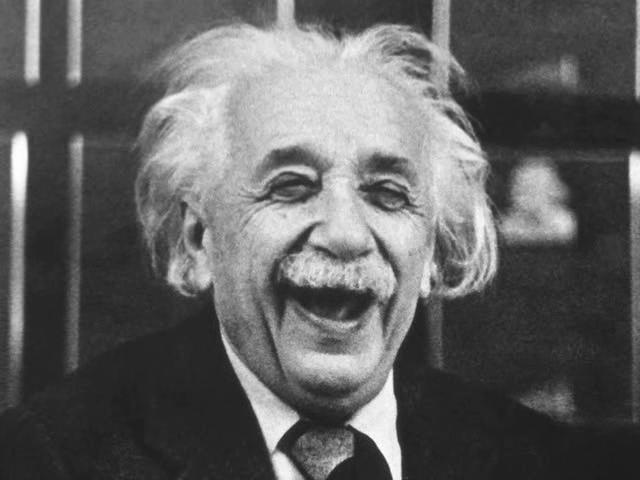
\includegraphics[width=0.4\textwidth]{einstein.jpeg}
 \label{Einstein}
 \end{figure}


\end{document}
